
\section{缩放选项}

有多种选项可控制或改变坐标轴的缩放。这里，“缩放”通常意味着两个方面：第一，每个方向上的单位向量大小；第二，每个方向上显示的限值。两者共同控制坐标轴盒的大小。此外，坐标轴描述也会改变大小。不过，\PGFPlots{} 只缩放单位并确定限值。默认情况下它不缩放坐标轴描述，以保持文本与图形之间字号的一致性。

通常，人们只希望提供目标尺寸，而让 \PGFPlots{} 完成其余工作。这是默认行为；它将坐标轴缩放到 |width| 和 |height|。如果你提供了其中一个选项，则坐标轴会在保持纵横比的同时重新缩放。

有时，人们希望显式地提供单位向量，以确保一个单位占据预定的空间量。这可以通过 |x|、|y| 和 |z| 键来实现。在这种情况下，|width| 和 |height| 选项将被忽略（或仅应用于未指定的单位向量）。

另一种常见方法是强制指定特定的 |unit vector ratio|：例如使用 |axis equal| 指定每个单位应占据相同的空间量。在这里，\PGFPlots{} 统一缩放所有向量的长度，也就是说它对每个向量应用相同的缩放比例。这是通过 |scale mode| 配置实现的，它基本上是 |scale mode=stretch to fill| 或 |scale mode=scale uniformly| 之一：\PGFPlots{} 试图通过找到一个\emph{公共}缩放因子来满足预定的 |width| 和 |height| 参数。此外，它还尝试单独扩展现值以适应预定尺寸。

此外，你可以使用选项 |/pgfplots/scale| 简单地将所有最终单位按某个预定因子放大。这不会改变文本标签。

如果需要，你也可以向坐标轴提供 |/tikz/scale|。这将缩放整个最终图像，包括所有文本标签。


\subsection{常用缩放选项}

前面段落中提到的所有常用选项都在此描述。

\begin{pgfplotskey}{width=\marg{dimen} (initially empty)}
    将最终图片的宽度设置为 \marg{dimen}。

    任何非空尺寸，例如 |width=5cm|，都会设置所需的目标宽度。任何 \TeX{} 单位都被接受（例如 |200pt| 或 |5in|）。

    空值 |width={}| 表示“使用默认宽度，或按比例缩放到 |height|”。在这种情况下，\PGFPlots{} 使用 |\axisdefaultwidth| 的值作为目标量。不过，如果已经设置了 |height| 键，\PGFPlots{} 将以保持 |\axisdefaultwidth| 与 |\axisdefaultheight| 之间比例的方式重新缩放 |\axisdefaultwidth|。这允许只指定 |width| 和 |height| 之一，同时保持纵横比。

    因此，如果你只指定 |width=5cm| 而保留默认的 |height={}|，缩放将尊重初始纵横比。

    缩放会影响 $x$、$y$ 和 $z$ 的单位向量。它不会改变文本标签或坐标轴描述的大小。
    %
\begin{codeexample}[]
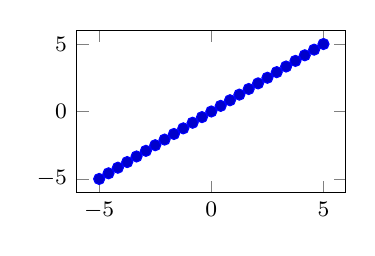
\begin{tikzpicture}
\begin{axis}[
    width=5cm,
]
    \addplot {x};
\end{axis}
\end{tikzpicture}
\end{codeexample}

    请注意，\PGFPlots{} 只是估算坐标轴标签和刻度标签所需的空间。该估算为坐标轴盒之外的所有内容假定了固定的空间量。这会导致最终图像可能比预定尺寸稍大或稍小。不过，这个固定量始终相同；它被设为 |45pt|。这意味着具有相同目标尺寸的多张图片，其坐标轴盒大小相同——即使描述所占的空间大小各不相同。

    也可以将\emph{坐标轴盒}缩放到预定的宽度/高度。在这种情况下，由于坐标轴描述，总宽度会更大。不过，坐标轴盒会精确填满所需的尺寸。
    %
\begin{codeexample}[]
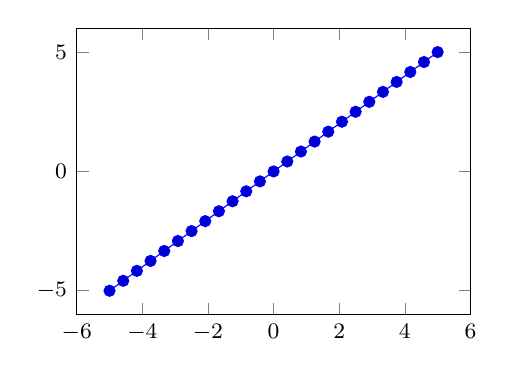
\begin{tikzpicture}
\begin{axis}[
    width=5cm,
    scale only axis,
]
    \addplot {x};
\end{axis}
\end{tikzpicture}
\end{codeexample}

    \paragraph{注意：}

    更改 |width| 和/或 |height| \emph{只} 改变单位向量的大小。特别是，它不会改变任何坐标轴描述的字号，也不会改变相邻刻度标签之间的默认间距。最佳实践是将 |width|/|height| 用于“小”更改，也就是字号应保持不变的更改。如果你需要不同的缩放“品质”，请考虑使用 styles |normalsize|、|small|、|footnotesize| 或 |tiny|（在 page~\pageref{sec:scaling:styles} 的 Section~\ref{sec:scaling:styles} 中描述），\emph{然后}再更改为你所需的尺寸。

    \begin{command}{\axisdefaultwidth}
        此宏定义默认宽度。它被预设为 |240pt|。

        此默认宽度定义了纵横比，只要只指定 |width| 或 |height| 之一，就会使用该纵横比：纵横比即 |\axisdefaultwidth| 与 |\axisdefaultheight| 之比。

        你可以使用以下方式更改它：
        %
\begin{codeexample}[code only]
\def\axisdefaultwidth{10cm}
\end{codeexample}
    \end{command}
\end{pgfplotskey}

\begin{pgfplotskey}{height=\marg{dimen} (initially empty)}
    其工作方式与 |width| 相同，区别在于空值 |height={}| 默认“使用 |\axisdefaultheight|，或者如果只更改了 |width| 则按比例缩放”。

    \begin{command}{\axisdefaultheight}
        此宏定义默认高度。它被预设为 |207pt|。

        参见 |\axisdefaultwidth|。
    \end{command}
\end{pgfplotskey}

\begin{pgfplotskey}{scale only axis=\mchoice{true,false} (initially false)}
    如果启用了 |scale only axis|，则 |width| 和 |height| 仅应用于坐标轴矩形。因此，生成的图形比 |width| 和 |height| 大（因为有任何坐标轴描述）。不过，坐标轴盒精确具有预定的目标尺寸。

    如果 |scale only axis=false|（默认），\PGFPlots{} 将试图生成\emph{包含}标签、标题和刻度在内的所需宽度。
\end{pgfplotskey}

\begin{pgfplotsxykeylist}{%
    \x=\marg{dimen} (initially empty),
    \x={\{(\meta{x},\meta{y})\}}%
}
        \index{x!Assign unit vector}%
        \index{y!Assign unit vector}%
        \index{z!Assign unit vector}%
        \index{Unit vector!Assign}%
        \index{3d view!Assign unit vectors}%
        \index{View!Assign unit vectors}%
        允许指定目标单位向量中的零个、一个、两个或三个。

    在此上下文中，“单位向量”是一个二维向量，它定义了到画布上的投影：每个逻辑绘图坐标 $(x,y)$ 都绘制在画布位置
    %
        \begin{equation*}
            x \cdot
                \begin{bmatrix}
                    e_{xx} \\
                    e_{xy}
                \end{bmatrix}
                    + y \cdot
                        \begin{bmatrix}
                            e_{yx} \\
                            e_{yy}
                        \end{bmatrix}.
        \end{equation*}
    %
    单位向量 $e_x$ 和 $e_y$ 决定了当前（始终为二维）图像中的纸张位置。对于标准三维坐标轴，绘图坐标 $(x,y,z)$ 绘制在
    %
        \begin{equation*}
            x \cdot
                \begin{bmatrix}
                    e_{xx} \\
                    e_{xy}
                \end{bmatrix}
                    + y \cdot
                        \begin{bmatrix}
                            e_{yx} \\
                            e_{yy}
                        \end{bmatrix}
                            + z \cdot
                                \begin{bmatrix}
                                    e_{zx} \\
                                    e_{zy}
                                \end{bmatrix}.
        \end{equation*}

    初始设置为这些键中的每一个都赋值为空，即 |x={},y={},z={}|。在这种情况下，\PGFPlots{} 可以自由地选择这些向量。为此，它会使用 |width|、|height|、|scale mode|、|plot box ratio|、|unit vector ratio|、|view| 以及坐标轴限值。

    键 |x=|\marg{dimen} 只是设置 $e_x = (\text{dimen},0)^T$，而 |y=|\marg{dimen} 设置 $e_y = (0,\text{dimen})^T$。使用 |z=|\marg{dimen} 会得到 $e_z = (\text{dimen},\text{dimen})^T$。在此上下文中，\meta{dimen} 是任何 \TeX{} 尺寸，例如 |1mm|、|2cm| 或 |5pt|。请注意，你不应对 \meta{dimen} 使用负值（请考虑使用 |x dir| 及其变体来反转坐标轴方向）。
    %
\begin{codeexample}[]
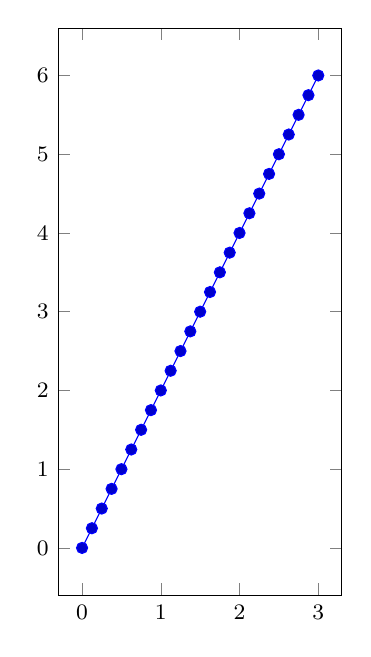
\begin{tikzpicture}
\begin{axis}[
    x=1cm,
    y=1cm,
]
    \addplot expression [domain=0:3] {2*x};
\end{axis}
\end{tikzpicture}
\end{codeexample}

\begin{codeexample}[]
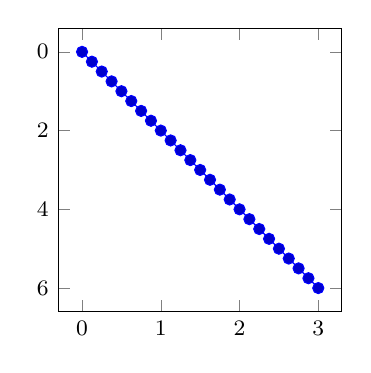
\begin{tikzpicture}
\begin{axis}[
    x=1cm,
    y=0.5cm,
    y dir=reverse,
]
    \addplot expression [domain=0:3] {2*x};
\end{axis}
\end{tikzpicture}
\end{codeexample}

    请注意，如果你只更改一个方向的单位向量，其他向量将由 \PGFPlots{} 选择——并被缩放，以尽 \PGFPlots{} 所能填满预定的 |width| 和 |height|（但参见本键末尾关于三维绘图的说明）。
    %
\begin{codeexample}[]
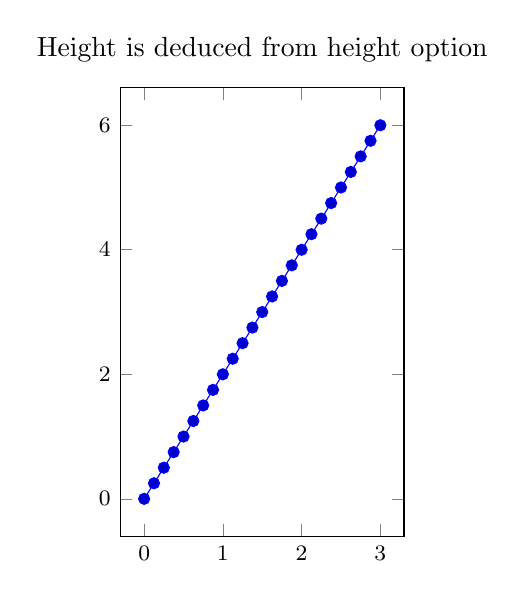
\begin{tikzpicture}
\begin{axis}[
    x=1cm,
    title=Height is deduced from height option,
]
    \addplot expression [domain=0:3] {2*x};
\end{axis}
\end{tikzpicture}
\end{codeexample}

    第二种语法 |x={(|\meta{x}|,|\meta{y}|)}| 显式设置 $e_x = (\mathit{x},\mathit{y})^T$。\footnote{请注意，你需要在向量周围加额外的花括号。否则，逗号会被解释为下一个键值对的分隔符。} 对应的 |y| 和 |z| 键的工作方式类似。这允许定义倾斜或旋转的坐标轴。

\begin{codeexample}[]
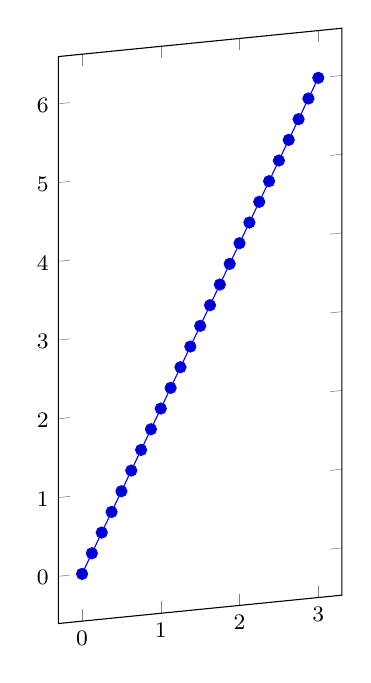
\begin{tikzpicture}
\begin{axis}[
    x={(1cm,0.1cm)},
    y=1cm,
]
    \addplot expression [domain=0:3] {2*x};
\end{axis}
\end{tikzpicture}
\end{codeexample}

\begin{codeexample}[]
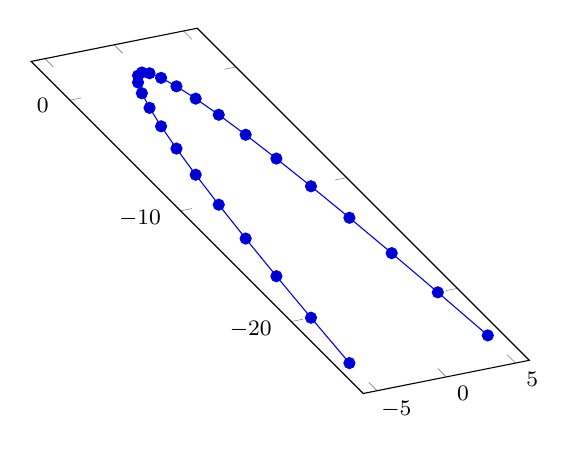
\begin{tikzpicture}
\begin{axis}[
    x={(5pt,1pt)},
    y={(-4pt,4pt)},
]
    \addplot {1-x^2};
\end{axis}
\end{tikzpicture}
\end{codeexample}

    为对数坐标轴设置 |x| 和/或 |y| 将设置用于 $1 \cdot e \approx 2.71828$（或任何被设为 |log basis x| 的值）的尺寸。

    请注意，\emph{不能} 将 |x| 指定为 |tikzpicture| 的参数。以下选项
    %
\begin{codeexample}[code only]
\begin{tikzpicture}[x=1.5cm]
\begin{axis}
    ...
\end{axis}
\end{tikzpicture}
\end{codeexample}
    %
    不会产生任何效果，因为坐标轴会重新缩放其坐标（参见 |width| 选项）。

    请注意，显式提供单位向量通常会导致 \PGFPlots{} 忽略任何其他缩放选项。换句话说：如果你写 |y=0.1cm|，\PGFPlots{} 将使用 $(0\text{cm},0.1\text{cm})$ 作为 $y$ 投影向量。不过，如果你添加 |scale mode=scale uniformly|，你就允许 \PGFPlots{} 更改向量的\emph{长度}。当然，它会保持它们的相对方向和相对大小。在这种情况下，\PGFPlots{} 将试图确定一个合适的公共缩放因子，\emph{并且}它还会试图更改坐标轴限值以填满预定的 |width| 和 |height|（详见 |scale mode| 的文档）。
    %
\begin{codeexample}[]
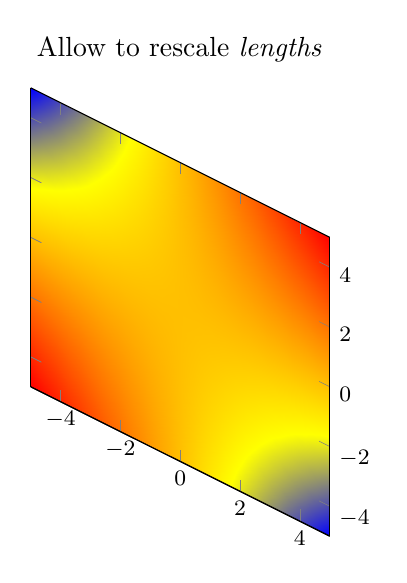
\begin{tikzpicture}
\begin{axis}[
    title=Allow to rescale \emph{lengths},
    x={(0.1cm,-0.05cm)},
    y=0.1cm,
    z=0cm,
    axis on top,
    scale mode=scale uniformly,
]
    \addplot3 [surf,shader=interp] {x*y};
\end{axis}
\end{tikzpicture}
\end{codeexample}
    %
    \noindent 在上面的例子中，\PGFPlots{} 决定只重新缩放单位——代价是牺牲了 |width| 约束。


    \paragraph{字号更改：}

    如果你想以简单的方式更改字号或刻度标签的密度，另见 Section~\ref{sec:scaling:styles}。


    \paragraph{三维坐标轴的显式单位：}

    从版本 1.5 开始，也可以为三维坐标轴提供单位向量。在这种情况下，需要满足以下额外假设：
    %
    \begin{enumerate}
        \item 如果你想控制三维单位，你需要提供 |x|、|y| 和 |z| 键的\emph{全部}。对于二维坐标轴，也支持只提供 |x| 或 |y| 之一。
        \item 任何提供的三维单位向量都被假定构成一个\emph{右手坐标系}。换句话说：伸出你的右手，让拇指指向 |x| 方向，食指指向 |y| 方向，中指指向 |z| 方向。如果做不到这一点，\PGFPlots{} 的输出将会出错。做出此假设的原因是 \PGFPlots{} 需要根据提供的单位计算视图方向（见下文）。

            如果你想反转方向，请考虑使用 |x dir=reverse| 或其变体。
        \item 对于三维坐标轴，\PGFPlots{} 根据提供的单位向量计算一个视图方向。视图方向是启用 |z buffer| 功能所必需的（也就是说，用于判断深度）。\footnote{\PGFPlots{} 提供了一个名为 \texttt{view dir=\marg{x}\marg{y}\marg{z}} 的调试选项，可用于覆盖视图方向，如果将来有此需要的话。}
    \end{enumerate}
    %
    此特性用于 \verbpdfref{\addplot3 graphics} 功能，对比 Section~\ref{sec:plotgraphics3d} 在 page~\pageref{sec:plotgraphics3d} 上的例子。


    \paragraph{限制：}

    遗憾的是，倾斜坐标轴\textbf{不能用于条形图}。
        \index{Errors!Skewed axes and bar plots}%
        \index{Bar Plots!Skewed axes problems}%
\end{pgfplotsxykeylist}

\begin{pgfplotsxykey}{\x mode=\mchoice{normal,linear,log} (initially normal)}
    允许为每个 $x,y,z$ 组合在线性（=normal）或对数坐标轴缩放之间进行选择，或选择对数绘图。

    对数绘图使用 |log basis x| 及其变体的当前设置来确定底数（默认是 $e$）。
    % FIXME : replicated in pgfplots.reference.specifyrange.tex
\end{pgfplotsxykey}

{\def\pgfmanualpdflabel#1#2{}
\begin{pgfplotsxykey}{\x\ dir=\mchoice{normal,reverse} (initially normal)}
    允许反转坐标轴方向，使值按递减顺序给出。

    这些键在 page~\pageref{key:pgfplots:xydir} 上有详尽的文档。
\end{pgfplotsxykey}
}

\begin{pgfplotskey}{axis equal=\marg{true,false} (initially false)}
    每个单位向量被设置为相同长度，而坐标轴尺寸保持不变。此后，$x$ 和 $y$ 中每个单位的大小比将相同。

    坐标轴限值会被扩大以补偿缩放效果。
    %
\begin{codeexample}[]
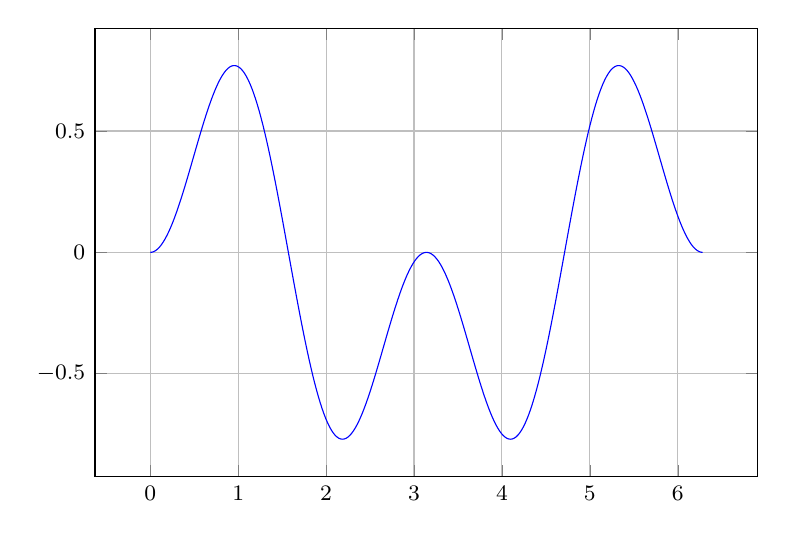
\begin{tikzpicture}
    \begin{axis}[axis equal=false,grid=major]
        \addplot [blue] expression [domain=0:2*pi,samples=300] {sin(deg(x))*sin(2*deg(x))};
    \end{axis}
\end{tikzpicture}
    \hspace{1cm}
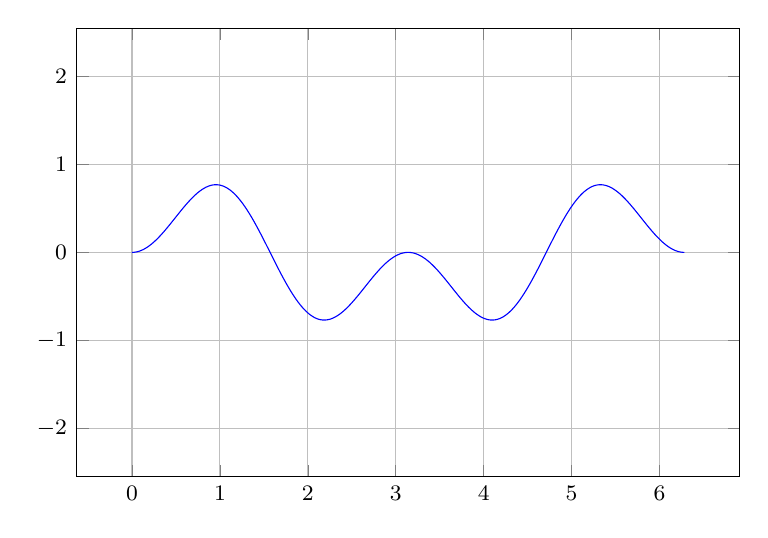
\begin{tikzpicture}
    \begin{axis}[axis equal=true,grid=major]
        \addplot [blue] expression [domain=0:2*pi,samples=300] {sin(deg(x))*sin(2*deg(x))};
    \end{axis}
\end{tikzpicture}
\end{codeexample}

\begin{codeexample}[]
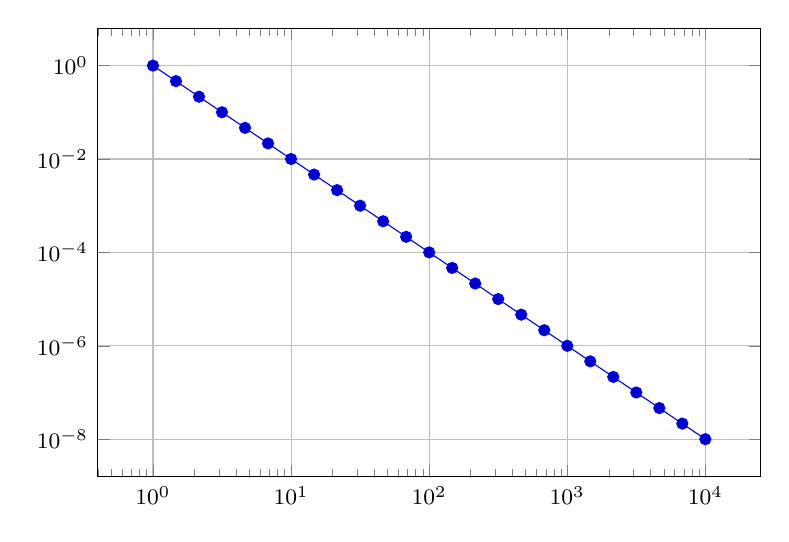
\begin{tikzpicture}
    \begin{loglogaxis}[axis equal=false,grid=major]
        \addplot expression [domain=1:10000] {x^-2};
    \end{loglogaxis}
\end{tikzpicture}
    \hspace{1cm}
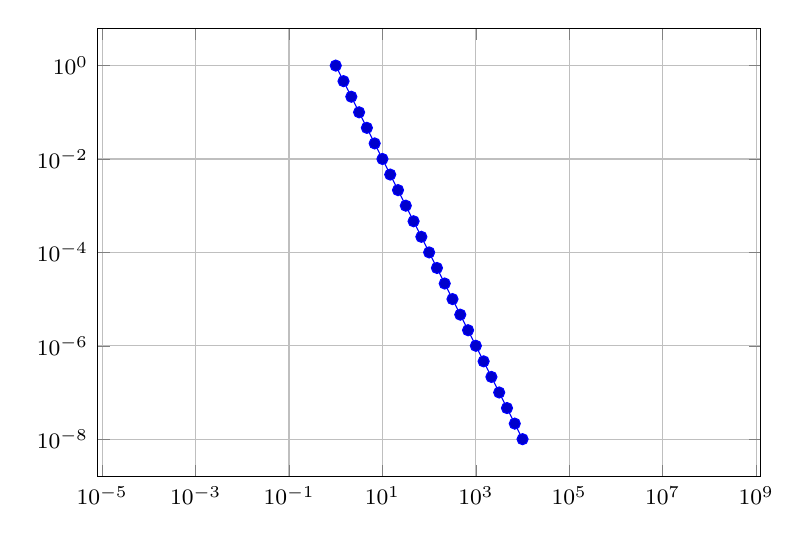
\begin{tikzpicture}
    \begin{loglogaxis}[axis equal=true,grid=major]
        \addplot expression [domain=1:10000] {x^-2};
    \end{loglogaxis}
\end{tikzpicture}
\end{codeexample}

\message{'warning /pgfplots/warning/approx empty range enlarged' is expected here.^^J}%
\begin{codeexample}[]
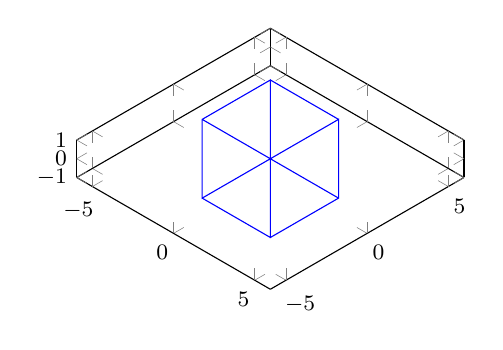
\begin{tikzpicture}
\begin{axis}[axis equal,small,view={45}{35.26}]
    \addplot3 [mark=cube, blue, mark size=1cm]
        coordinates {(0,0,0)};
\end{axis}
\end{tikzpicture}
\end{codeexample}

    配置 |axis equal=true| 实际上只是一个样式，它设置
    |unit vector ratio=1 1 1,unit rescale|\allowbreak| keep size=true|。
\end{pgfplotskey}

\begin{pgfplotskey}{axis equal image=\marg{true,false} (initially false)}
    与 |axis equal| 类似，但坐标轴限值也保持不变（导致图像更小）。
    %
\begin{codeexample}[]
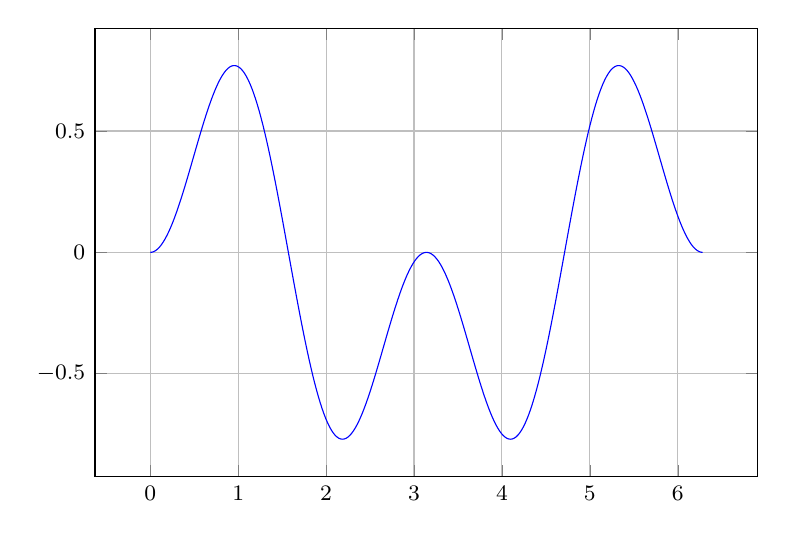
\begin{tikzpicture}
    \begin{axis}[axis equal image=false,grid=major]
        \addplot [blue] expression [domain=0:2*pi,samples=300] {sin(deg(x))*sin(2*deg(x))};
    \end{axis}
\end{tikzpicture}
    \hspace{1cm}
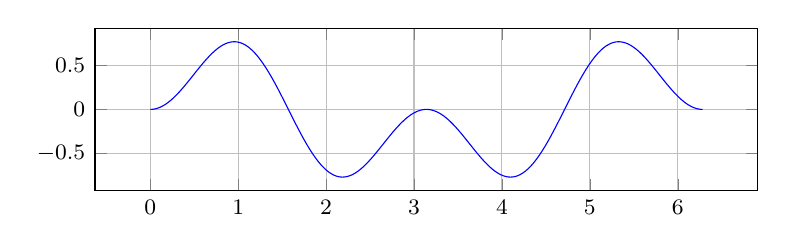
\begin{tikzpicture}
    \begin{axis}[axis equal image=true,grid=major]
        \addplot [blue] expression [domain=0:2*pi,samples=300] {sin(deg(x))*sin(2*deg(x))};
    \end{axis}
\end{tikzpicture}
\end{codeexample}

\begin{codeexample}[]
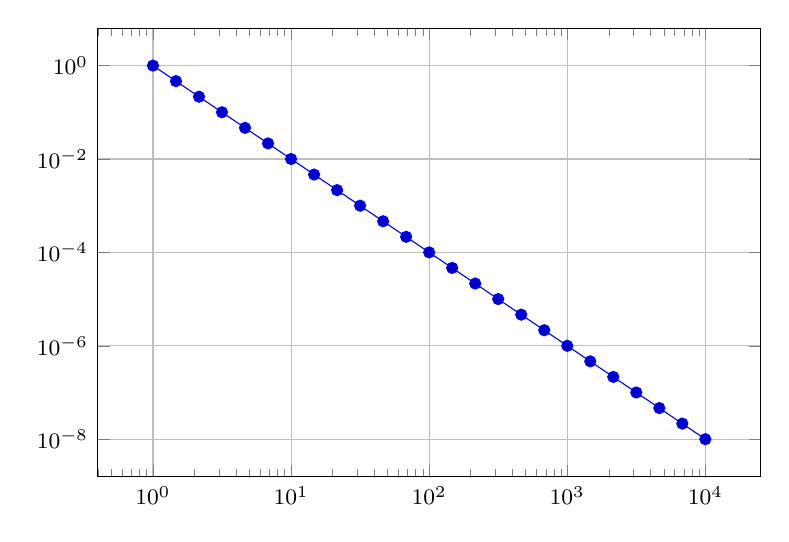
\begin{tikzpicture}
    \begin{loglogaxis}[axis equal image=false,grid=major]
        \addplot expression [domain=1:10000] {x^-2};
    \end{loglogaxis}
\end{tikzpicture}
\hspace{1cm}
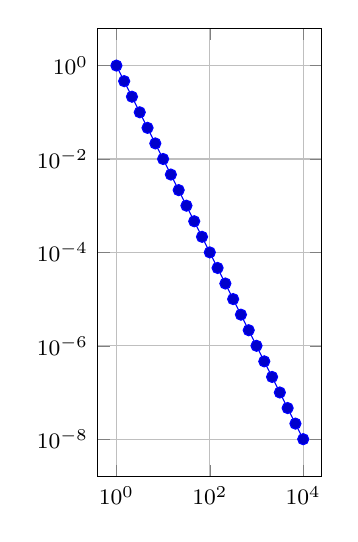
\begin{tikzpicture}
    \begin{loglogaxis}[axis equal image=true,grid=major]
        \addplot expression [domain=1:10000] {x^-2};
    \end{loglogaxis}
\end{tikzpicture}
\end{codeexample}
    %
    配置 |axis equal image=true| 实际上只是一个样式，它设置
    |unit vector ratio=1 1 1,unit rescale|\allowbreak| keep size=false|。
\end{pgfplotskey}

\begin{pgfplotskey}{unit vector ratio=\marg{rx ry rz} (initially empty)}
    允许提供自定义的单位向量比。

    此键允许告诉 \PGFPlots{}，例如，$x$ 方向上的一个单位应该是 $y$ 方向上一个单位的两倍长：
    %
\begin{codeexample}[]
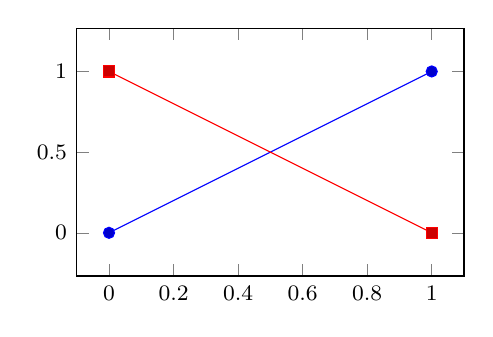
\begin{tikzpicture}
\begin{axis}[unit vector ratio=2 1,small]
    \addplot coordinates {(0,0) (1,1)};
    \addplot table [row sep=\\,col sep=&] {
        x & y \\
        0 & 1 \\
        1 & 0 \\
    };
\end{axis}
\end{tikzpicture}
\end{codeexample}
    %
    \noindent 提供 |unit vector ratio=2 1| 意味着 $\frac{||e_x||}{||e_y||} = 2$，其中每个坐标 $(x,y)$ 放置在 $x e_x + y e_y \in \R^2$ 处（参见 |x| 和 |y| 选项的文档）。请注意，|axis equal| 不过就是 |unit vector ratio=1 1 1|。

    参数 \meta{rx}、\meta{ry} 和 \meta{rz} 分别是 $x$、$y$ 和 $z$ 向量的比。对于二维坐标轴，只考虑 \meta{rx} 和 \meta{ry}；它们是相对于 $y$ 坐标轴给出的。换句话说：$x$ 单位向量将是 $y$ 单位向量的 \meta{rx}$/$\meta{ry} 倍长。对于三维坐标轴，可以提供全部三个参数；它们是相对于 $z$ 单位向量解释的。因此，一个 |unit vector ratio=1 2 4| 的三维坐标轴，其 $x$ 单位长度为 $z$ 单位的 $\nicefrac 14$，$y$ 单位长度为 $z$ 单位的 $\nicefrac24$。

    末尾的 |1| 值可以省略，也就是说 |unit vector ratio=2 1| 与 |unit vector ratio=2| 相同；而 |unit vector ratio=3 2 1| 与 |unit vector ratio=3 2| 相同。空值 |unit vector ratio={}| 会禁用单位向量重新缩放。

    请注意，激活的 |unit vector ratio| 会隐式设置 |scale mode=scale uniformly|。\footnote{这是在版本 1.6 中引入的。对于更早的版本，axis equal 功能对三维坐标轴会产生错误的结果。}

    \begin{pgfplotskeylist}{%
        unit vector ratio*=\marg{rx ry rz},
        unit rescale keep size=\mchoice{%
                true,
                false,
                unless limits declared%
            } (initially unless limits declared)%
    }
    \label{key:unit:rescale:keep:size}
        在默认配置下，\PGFPlots{} 会保持原始坐标轴尺寸，即使 |unit vector ratio| 涉及不同的缩放。

        它通过扩展现值来做到这一点。
        %
\begin{codeexample}[]
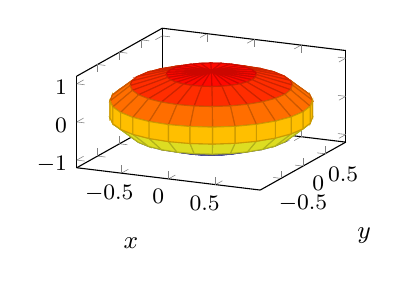
\begin{tikzpicture}
    \begin{axis}[footnotesize,xlabel=$x$,ylabel=$y$,unit vector ratio=]
        \addplot3 [surf,z buffer=sort,samples=15,
            variable=\u, variable y=\v,
            domain=0:180, y domain=0:360]
               ({cos(u)*sin(v)}, {sin(u)*sin(v)}, {cos(v)});
    \end{axis}
\end{tikzpicture}
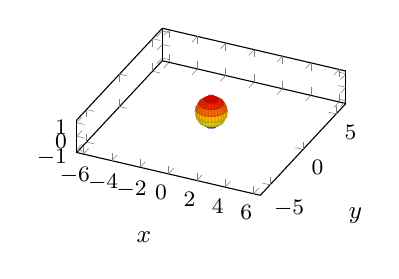
\begin{tikzpicture}
    \begin{axis}[footnotesize,xlabel=$x$,ylabel=$y$,unit vector ratio=1 1 1]
        \addplot3 [surf,z buffer=sort,samples=15,
            variable=\u, variable y=\v,
            domain=0:180, y domain=0:360]
               ({cos(u)*sin(v)}, {sin(u)*sin(v)}, {cos(v)});
    \end{axis}
\end{tikzpicture}
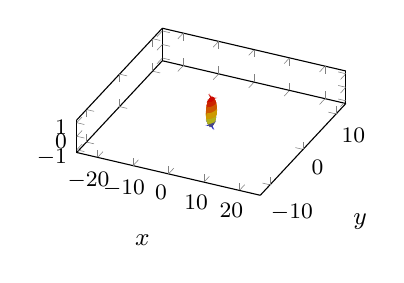
\begin{tikzpicture}
    \begin{axis}[footnotesize,xlabel=$x$,ylabel=$y$,unit vector ratio=0.25 0.5]
        \addplot3 [surf,z buffer=sort,samples=15,
            variable=\u, variable y=\v,
            domain=0:180, y domain=0:360]
               ({cos(u)*sin(v)}, {sin(u)*sin(v)}, {cos(v)});
    \end{axis}
\end{tikzpicture}
\end{codeexample}
        %
        \noindent 上面的例子是同一张图，使用了三种不同的单位比。第一种没有限值限制（这是默认配置）。第二种为每个单位向量使用相同长度，并扩展现值以保持相同尺寸。第三个例子中，$x$ 单位长度为 $z$ 单位的 $\nicefrac14$，$y$ 单位长度为 $z$ 单位的 $\nicefrac12$。

        \PGFPlots{} 尽最大努力尊重所涉及的缩放选项（预定的 |width| 和 |height|、|unit vector ratio| 以及任何指定的坐标轴限值）。在上面的例子中，它扩大了水平限值，并保持 $z$ 限值不变。关于所涉及的算法及其参数的详细信息，参见 |scale mode| 及其文档。

        键 |unit rescale keep size=false|，或者等价地 |unit vector ratio*=...|，不会扩展现值：
        %
\begin{codeexample}[]
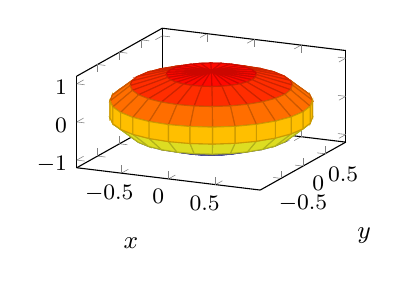
\begin{tikzpicture}
    \begin{axis}[footnotesize,xlabel=$x$,ylabel=$y$,unit vector ratio=]
        \addplot3 [surf,z buffer=sort,samples=15,
            variable=\u, variable y=\v,
            domain=0:180, y domain=0:360]
               ({cos(u)*sin(v)}, {sin(u)*sin(v)}, {cos(v)});
    \end{axis}
\end{tikzpicture}
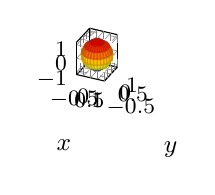
\begin{tikzpicture}
    \begin{axis}[footnotesize,xlabel=$x$,ylabel=$y$,
        unit rescale keep size=false,
        unit vector ratio=1 1 1]
        \addplot3 [surf,z buffer=sort,samples=15,
            variable=\u, variable y=\v,
            domain=0:180, y domain=0:360]
               ({cos(u)*sin(v)}, {sin(u)*sin(v)}, {cos(v)});
    \end{axis}
\end{tikzpicture}
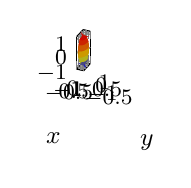
\begin{tikzpicture}
    \begin{axis}[footnotesize,xlabel=$x$,ylabel=$y$,
        unit vector ratio*=0.25 0.5, % the '*' implies 'unit rescale keep size=false'
    ]
        \addplot3 [surf,z buffer=sort,samples=15,
            variable=\u, variable y=\v,
            domain=0:180, y domain=0:360]
               ({cos(u)*sin(v)}, {sin(u)*sin(v)}, {cos(v)});
    \end{axis}
\end{tikzpicture}
\end{codeexample}
        %
        键 |unit rescale keep size| 还会影响 |scale mode=scale uniformly|（它与 |axis equal| 密切相关）。

        下面是 |unit rescale keep size| 值的参考：值 \declaretext{true} 表示 \PGFPlots{} 将扩展现值以保持尺寸。它会尽量尊重用户提供的限值，但如果用户提供了\emph{所有}限值，它将\emph{覆盖}用户提供的限值并重新缩放它们。因此，|true| 将坐标轴尺寸的优先级置于用户提供的限值之上。选项 \declaretext{false} 永远不会重新缩放坐标轴限值。选项 \declaretext{unless limits declared} 是一种混合：它会扩展现值，除非用户提供了它们。如果用户显式提供了所有限值，此选项与 |false| 相同。
    \end{pgfplotskeylist}
\end{pgfplotskey}

\begin{pgfplotsxykeylist}{%
    \x\ post scale=\marg{scale} (initially empty),
    scale=\marg{scale} (initially empty)%
}
    让 \PGFPlots{} 根据 |width|、|height|、|view|、|plot box ratio|、|axis equal| 或使用 |x|、|y|、|z| 的显式单位向量计算坐标轴缩放，并根据 \meta{scale} \emph{重新缩放}得到的向量。

    |scale| 键将所有三个键设置为相同的 \meta{uniform scale} 值。这实际上等同于重新缩放整个坐标轴（但不改变描述的大小）。

    其他键允许单独重新缩放坐标轴。
    %
\begin{codeexample}[]
\begin{tikzpicture}
    \begin{axis}[y post scale=1]
        \addplot {x};
    \end{axis}
\end{tikzpicture}
\begin{tikzpicture}
    \begin{axis}[y post scale=2]
        \addplot {x};
    \end{axis}
\end{tikzpicture}
\end{codeexample}
    %
    因此，坐标轴变得\emph{更大}。这会覆盖任何先前的缩放。

\begin{codeexample}[]
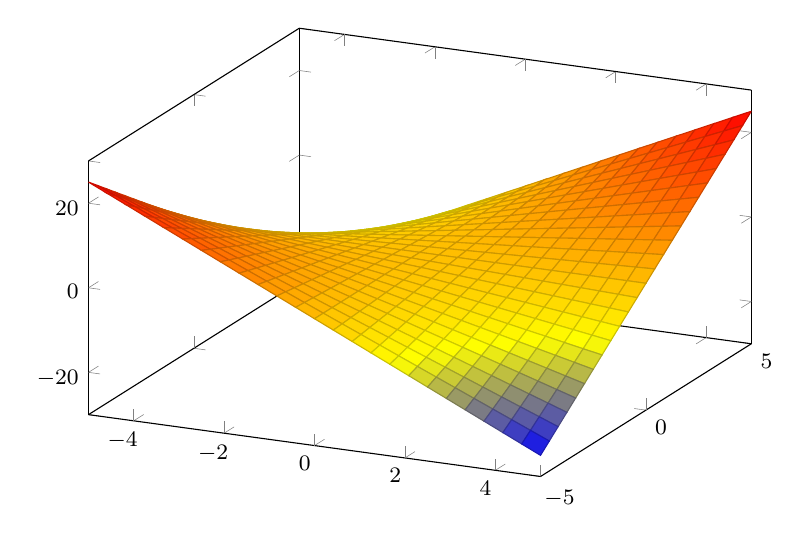
\begin{tikzpicture}
    \begin{axis}[z post scale=1]
        \addplot3 [surf] {x*y};
    \end{axis}
\end{tikzpicture}
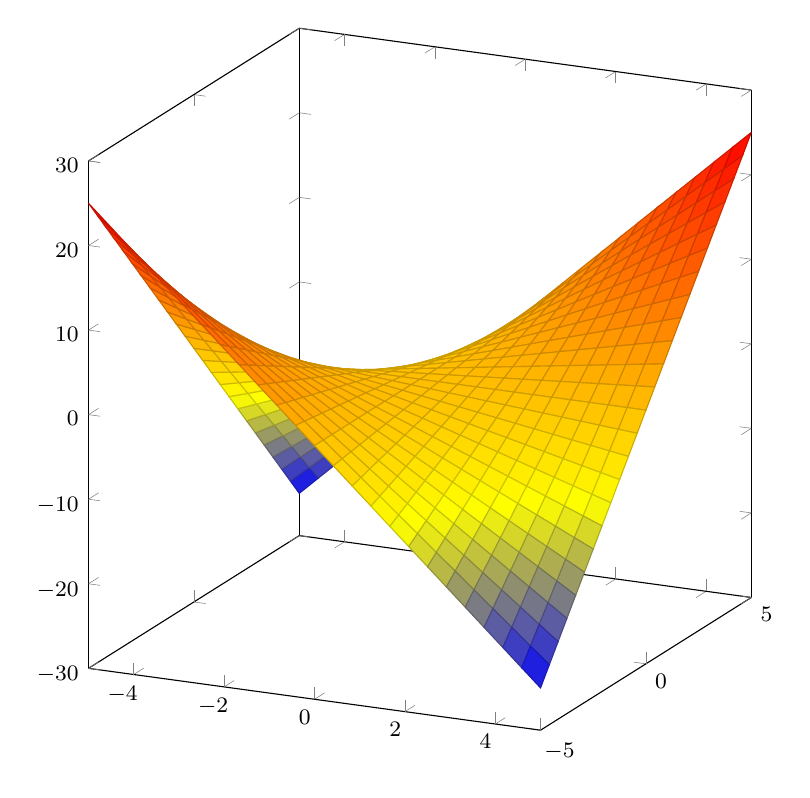
\begin{tikzpicture}
    \begin{axis}[z post scale=2]
        \addplot3 [surf] {x*y};
    \end{axis}
\end{tikzpicture}
\end{codeexample}
\end{pgfplotsxykeylist}


\subsection{缩放描述：预定义样式}
\label{sec:scaling:styles}

更改字号、标记大小等与整体绘图大小一起进行是合理的：大的绘图也应该有更大的字号，而小的绘图应该有小字号和更小的刻度间距。

\begin{keylist}{%
    /tikz/font=\mchoice{%
        \textbackslash normalfont,
        \textbackslash small,
        \textbackslash tiny,
        $\dotsc$%
    },
    /pgfplots/max space between ticks=\marg{integer},
    /pgfplots/try min ticks=\marg{integer},
    /tikz/mark size=\marg{integer}%
}
    这些键应根据图形的尺寸进行调整。使用以下方式
    %
\begin{codeexample}[code only]
\pgfplotsset{
    tick label style={font=\footnotesize},
    label style={font=\small},
    legend style={font=\small},
}
\end{codeexample}
    %
    为不同的描述提供不同的字体。

    键 |max space between ticks| 和 |try min ticks| 在 page~\pageref{maxspacebetweenticks} 上描述，它们配置连续刻度标签之间的近似距离和数量（以 |pt| 为单位）。请在此处省略 |pt| 后缀。
\end{keylist}

有几个预定义的缩放样式可设置其中一些选项：

\begin{stylekey}{/pgfplots/normalsize}
    重新初始化 \PGFPlots{} 的标准缩放选项。
    %
\begin{codeexample}[]
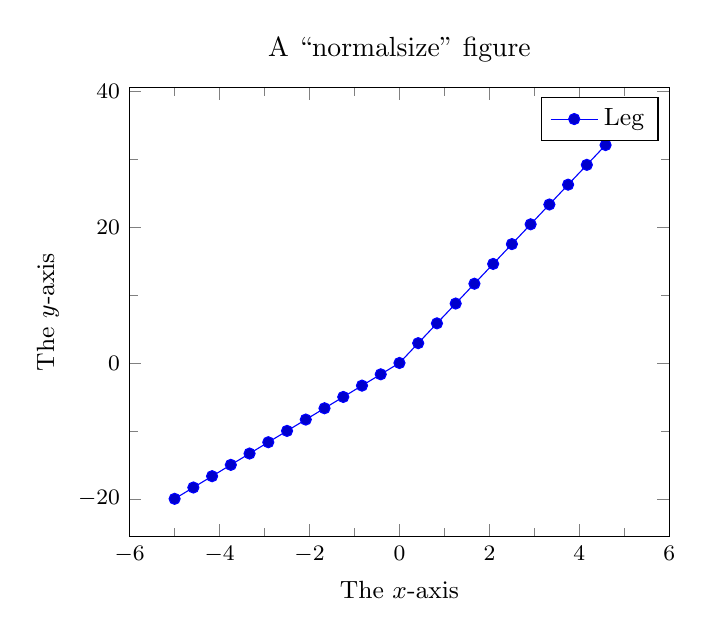
\begin{tikzpicture}
    \begin{axis}[normalsize,
        title=A ``normalsize'' figure,
        xlabel=The $x$-axis,
        ylabel=The $y$-axis,
        minor tick num=1,
        legend entries={Leg},
    ]
        \addplot {max(4*x,7*x)};
    \end{axis}
\end{tikzpicture}
\end{codeexample}

    初始设置是
\begin{codeexample}[code only]
\pgfplotsset{
    normalsize/.style={
        /pgfplots/width=240pt,
        /pgfplots/height=207pt,
        /pgfplots/max space between ticks=35,
    },
}
\end{codeexample}
\end{stylekey}

\begin{stylekey}{/pgfplots/small}
    重新定义若干键，使坐标轴“更小”。
    %
\begin{codeexample}[]
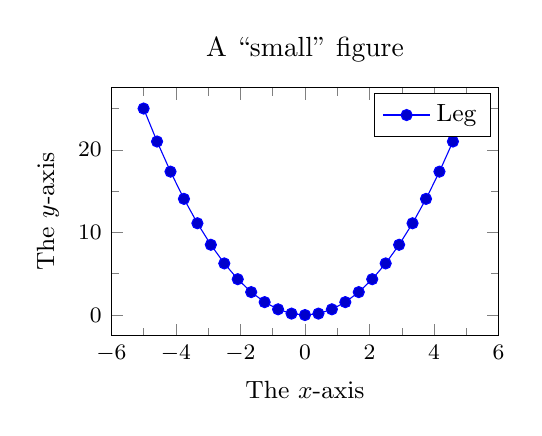
\begin{tikzpicture}
\begin{axis}[
    small,
    title=A ``small'' figure,
    xlabel=The $x$-axis,
    ylabel=The $y$-axis,
    minor tick num=1,
    legend entries={Leg},
]
    \addplot {x^2};
\end{axis}
\end{tikzpicture}
\end{codeexample}
    %
    初始设置是
    %
\begin{codeexample}[code only]
\pgfplotsset{
    small/.style={
        width=6.5cm,
        height=,
        tick label style={font=\footnotesize},
        label style={font=\small},
        max space between ticks=25,
    },
}
\end{codeexample}
    %
    欢迎你重新定义缩放——此选项在不必输入太多内容就能获得更多刻度方面仍然有用。例如，你可以设置 |small,width=6cm|。
\end{stylekey}

\begin{stylekey}{/pgfplots/footnotesize}
    重新定义若干键，使坐标轴更小。刻度标签将使用 |\footnotesize|。
    %
\begin{codeexample}[]
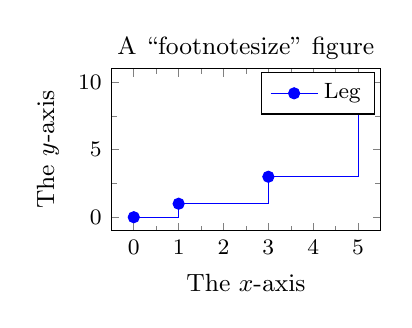
\begin{tikzpicture}
\begin{axis}[
    footnotesize,
    title=A ``footnotesize'' figure,
    xlabel=The $x$-axis,
    ylabel=The $y$-axis,
    minor tick num=1,
    legend entries={Leg},
]
    \addplot+ [const plot] coordinates {
        (0,0) (1,1) (3,3) (5,10)
    };
\end{axis}
\end{tikzpicture}
\end{codeexample}
    %
    初始设置是
    %
\begin{codeexample}[code only]
\pgfplotsset{
    footnotesize/.style={
        width=5cm,
        height=,
        legend style={font=\footnotesize},
        tick label style={font=\footnotesize},
        label style={font=\small},
        title style={font=\small},
        every axis title shift=0pt,
        max space between ticks=15,
        every mark/.append style={mark size=8},
        major tick length=0.1cm,
        minor tick length=0.066cm,
    },
}
\end{codeexample}
    %
    与 |small| 一样，可以先设置 |footnotesize|，然后再设置 |width|，这样会很方便。

    你需要 |compat=1.3| 或更新版本才能使其生效。
\end{stylekey}

\begin{stylekey}{/pgfplots/tiny}
    重新定义若干键，使坐标轴非常小。大多数描述将使用 |\tiny| 作为字号。
    %
\begin{codeexample}[]
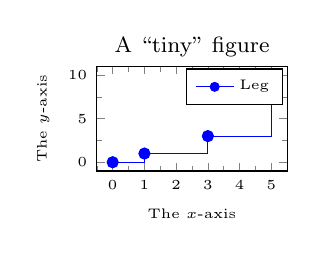
\begin{tikzpicture}
\begin{axis}[tiny,
    title=A ``tiny'' figure,
    xlabel=The $x$-axis,
    ylabel=The $y$-axis,
    minor tick num=1,
    legend entries={Leg},
]
    \addplot+ [const plot] coordinates {
        (0,0) (1,1) (3,3) (5,10)
    };
\end{axis}
\end{tikzpicture}
\end{codeexample}
    %
    初始设置是
    %
\begin{codeexample}[code only]
\pgfplotsset{
    tiny/.style={
        width=4cm,
        height=,
        legend style={font=\tiny},
        tick label style={font=\tiny},
        label style={font=\tiny},
        title style={font=\footnotesize},
        every axis title shift=0pt,
        max space between ticks=12,
        every mark/.append style={mark size=6},
        major tick length=0.1cm,
        minor tick length=0.066cm,
        every legend image post/.append style={scale=0.8},
    },
}
\end{codeexample}
    %
    与 |small| 一样，可以使用 |tiny,width=4.5cm| 来调整宽度。

    你需要 |compat=1.3| 或更新版本才能使其生效。
\end{stylekey}


\subsection{缩放策略}

本节内容相当复杂——而且通常你不需要了解它，因为默认情况下 \PGFPlots{} 会自动控制相关内容。你可以跳过本节。

\begin{pgfplotskey}{scale mode=\mchoice{auto,none,stretch to fill,scale uniformly} (initially auto)}
    指定如何选择（各自的）单位向量缩放因子、它们的长度比，以及可能的坐标轴限值，以填满预定的 |width| 和 |height|。

    |scale mode| 的实现期望有一组“初始”单位向量。这组初始单位向量的确定方式如下：对于标准二维坐标轴，它就是单位立方体 $e_x=(1\text{pt},0\text{pt})^T$、$e_y=(0\text{pt},1\text{pt})^T$、$e_z=0$。对于三维坐标轴，它是 |view| 和 |plot box ratio| 这两个键的结果。如果你通过 |x|、|y| 或 |z| 之一显式提供了单位，则该值就是初始单位向量。

    此外，它还期望有“初始”坐标轴限值（即 |xmin|、|xmax| 等的值）。初始坐标轴限值是那些从你的数据推导出来的限值，或者是显式提供的限值。此外，初始坐标轴限值已经包含了 |enlargelimits| 键的更改。

    给定初始单位向量集合和初始坐标轴限值，|scale mode| 的实现是一种“后处理器”，它生成修改后的单位向量和修改后的坐标轴限值，以满足所有指定的约束。这些约束是 |width|、|height| 和 |unit vector ratio|。

    初始选项 \declaretext{auto} 告诉 \PGFPlots{} 完全控制此键。它根据实际上下文选择其他可能选项之一。如果设置了 |unit vector ratio|，选项 |auto| 求值为 |scale uniformly|；否则它求值为 |stretch to fill|。

    选项 \declaretext{none} 完全不应用任何重新缩放。如果要使用 |x|、|y|（以及可能的 |z|）的预定长度，请使用此项。换句话说：它会忽略 |width| 和 |height|。在这种情况下，你可能需要设置 |x post scale| 及其变体来手动重新缩放单位。另见 |disabledatascaling|。

    选项 \declaretext{stretch to fill} 取初始单位向量，并使用\emph{两个}独立的缩放比例重新缩放单位向量：一个产生合适的 |width|，另一个产生合适的 |height|。因此，单位向量被修改和扭曲，使最终图像适合预定尺寸。这通常是人们所期望的，除非显式提供了单位方向。此模式不改变坐标轴限值。请注意，如果某个单位向量已被显式提供，\PGFPlots{} 不会更改它。它只会更改其余的坐标轴限值。此模式与 |axis equal| 或 |unit vector ratio| 相矛盾。

    选项 \declaretext{scale uniformly} 取初始单位向量，并对所有单位只应用\emph{一个}缩放因子。在这种情况下，|width| 和 |height| 只有\emph{一个}公共缩放因子。自然地，这会导致不令人满意的结果，因为最终宽度或最终高度之一将无法满足。因此，此选项会调整坐标轴限值以得到所需尺寸。这样，单位向量在缩放前的大小\emph{关系和角度}完全相同；只是它们的大小被统一改变。此外，坐标轴限值可能被更改（对每个坐标轴限值使用各自的缩放因子）。请注意，如果单位向量已被显式提供，\PGFPlots{} 仍然可以用此选项重新缩放它——它会保持相对方向和大小比。选项 |scale uniformly| 尽最大努力以“有用”的方式修改自由度。“有用”的确切含义由 |scale uniformly strategy| 键决定。

    \begin{pgfplotskey}{scale uniformly strategy=\mchoice{%
            auto,
            units only,
            change vertical limits,\\
            change horizontal limits%
        } (initially auto)%
    }
        |scale uniformly| 方法需要确定一个\emph{公共}缩放因子，用于重新缩放每个坐标轴\emph{单位}。此外，它允许\emph{每个坐标轴限值}一个缩放因子，也就是说最多三个。

        此搜索的约束是：我们希望满足 |width|/|height| 约束，尽可能少地重新缩放，并且我们不希望缩小限值（因为这可能会隐藏数据点）。

        选项 \declaretext{auto} 自动选择其他可能性之一。根据我们拥有的是二维还是三维，它会比较可用的方法，并选择不缩小限值且涉及最少重新缩放的那个（也就是说，它可能会比较其他策略的结果）。这是默认值。如果你保留选项 |auto|，就不必担心其余选项。请注意，手动提供的坐标轴限值不会被修改。

        选项 \declaretext{units only} 不会扩大坐标轴限值。它只会重新缩放单位。为此，它选择缩放因子，使\emph{较小}的目标尺寸按期望填满。换句话说：如果 |width| $<$ |height|，它将缩放以满足 |width| 约束。|height| 约束将被忽略。$>$ 的情况则反过来处理。选项 |units only| 通常产生方形坐标轴，因为它取初始单位向量集合（通常是单位盒）并用公共缩放因子缩放它们。因此，如果你想要一个带盒坐标轴，可以选择 |units only|。不过，你仍然可以手动更改坐标轴限值。

        选项 \declaretext{change vertical limits} 为单位向量选择一个公共缩放因子，以满足 |width|（！）约束。这个公共缩放因子类似于 |units only|——但 |units only| 也可以决定满足 |height| 约束，而 |change vertical limits| 将缩放单位向量以满足 |width|。为了满足 |height| 约束，|change vertical limits| 只修改垂直限值。对于二维坐标轴，这是 |ymin| 和 |ymax|。对于三维坐标轴，这是 |zmin| 和 |zmax|。显然，它有可能会\emph{缩小}显示范围——在这种情况下，图像的部分内容将被裁剪掉。此方法\emph{假定}垂直坐标轴未被旋转（也就是说，$e_{yx}=0$ 或 $e_{zx}=0$，视情况而定）。对于旋转的坐标轴，它会拒绝工作并回退到 |units only|。如果你希望图像（即实际内容）尽可能宽，请选择 |change vertical limits|。你可以修改 |width| 和 |height| 以改善其结果。请注意，手动指定的坐标轴限值不会被更改，详见下文。

        选项 \declaretext{change horizontal limits} 尝试类似的方法，但针对水平限值：它确定一个合适的缩放因子应用于所有单位向量，并修改水平坐标轴限值以满足其余约束。对于二维坐标轴，这相当简单，因为我们通常有 $e_{xy} = 0$（也就是说，$x$ 单位向量的 $y$ 分量为零）且 $e_{yx}=0$，这样 \PGFPlots{} 可以轻松更改坐标轴限值。如果二维坐标轴的 $x$ 单位有 $e_{xy} \neq 0$，则此方法不适用并回退到 |units only|。对于三维坐标轴，它假定 $z$ 向量未被旋转，也就是说 $e_{zy} = 0$，并试图更改 $x$ 和 $y$ 两者的限值。这个选项要复杂得多，因为在这里 $x$ 和 $y$ 分量是耦合的。因此，公共单位缩放因子以及 $x$ 和 $y$ 的两个相关坐标轴限值补偿因子也是紧密耦合的。\PGFPlots{} 迭代求解一个非线性方程组，以得到所有三个缩放的合适解。如果 |change vertical limits| 会裁剪掉部分图像（因为它缩小了显示范围），而你又不想更改 |width| 和 |height|，请使用此方法。选项 |change horizontal limits| 通常会在生成的图形中产生更多空白。但它不会裁剪掉内容。手动指定的坐标轴限值不会被更改，详见下文。
    \end{pgfplotskey}


    \paragraph{手动提供的坐标轴限值：}

    任何为 |xmin| 及其变体手动提供的参数都被视为不可变；\PGFPlots{} 不会更改它们。如果你指定 |xmin|，\PGFPlots{} 将只更改 |xmax|，反之亦然。如果你同时指定 |xmin| 和 |xmax|，\PGFPlots{} 将完全不更改 $x$ 限值。请注意，如果你同时指定 |xmin| 和 |xmax|，\PGFPlots{} 将直接跳过缩放并放弃约束。它不会试图通过更改 $y$ 限值来弥补缩放机会的缺失，例如。这样做的正面效果是，指定限值不会改变坐标轴的整体外观。对坐标轴限值允许的更改集合可以通过以下键配置。


    \paragraph{与 }|enlargelimits| 的交互：

    请注意，|enlargelimits| 和 |scale mode| 是相互独立的：|enlargelimits| 的结果被用作“初始坐标轴限值”，这些限值可能会被 |scale mode| 更改（即使你说了 |enlargelimits=false|）。关于这种交互的详细信息，参见 |enlargelimits| 的文档。

    \begin{pgfplotskey}{unit rescale keep size=\mchoice{%
            true,
            false,
            unless limits declared%
        } (initially unless limits declared)%
    }
        在默认配置 \declaretext{unless limits declared} 下，单位重新缩放可能会导致坐标轴限值发生变化，以保持图形尺寸不变。不过，只有那些未被手动声明的限值才会被重新缩放：如果你说 |xmin=1|，则只有 |xmax| 以及 $y$ 和 $z$ 的限值可以更改。

        设置 |unit rescale keep size=|\declaretext{false} 将\emph{完全禁用}对坐标轴限值的修改，也就是说坐标轴限值不会被重新缩放以补偿单位向量上的缩放。

        设置 |unit rescale keep size=|\declaretext{true} 将始终重新缩放限值，即使它们已被手动声明。

        此键主要影响 |scale mode=scale uniformly|。而后者又用于 |axis equal| 和 |\addplot3 graphics|。

        另见此键的附加文档以及 page~\pageref{key:unit:rescale:keep:size} 上的相关例子。
    \end{pgfplotskey}

    选项 |scale uniformly| 被隐式用于 |axis equal| 和 \verbpdfref{\addplot3 graphics} 功能，其例子参见 Section~\ref{sec:plotgraphics3d} 在 page~\pageref{sec:plotgraphics3d} 上的文档。请注意，常见情况是初始单位向量构成单位立方体（也就是说，缩放前的那些，见上文）。在这种情况下，|scale uniformly| 与 |axis equal| 相同。
\end{pgfplotskey}
